\documentclass[11pt,a4paper,twocolumn]{article}

% === Core Packages ===
\usepackage[margin=2cm]{geometry}
\usepackage[utf8]{inputenc}
\usepackage[T1]{fontenc}
\usepackage{times}
\usepackage{amsmath,amssymb}
\usepackage{graphicx}
\usepackage{booktabs}
\usepackage{float}
\usepackage{enumitem}
\usepackage{tikz}
\usepackage{pgfplots}
\pgfplotsset{compat=1.18}
\usetikzlibrary{arrows.meta,shapes.geometric,positioning,calc,decorations.markings,fit,backgrounds}

% === Citation (IEEE style) ===
\usepackage[numbers,sort&compress]{natbib}
\bibliographystyle{IEEEtranN}

% === Hyperref ===
\usepackage[hidelinks]{hyperref}
\usepackage{xurl}

% === Settings ===
\setlength{\parindent}{1em}
\setlength{\parskip}{0.3em}

% === Title ===
\title{\textbf{Red de Reputación Descentralizada:\\Un marco para la organización natural de la sociedad}}
\author{Pavel Kudrna\\Prague, Czechia\\Borrador v1 --- Marzo de 2026}
\date{}

\begin{document}
\maketitle

% ============================================================
% ABSTRACT
% ============================================================
\begin{abstract}
El sentido de justicia---la convicción de que los agravios se reparan y el mérito se recompensa---es la fuerza cohesiva más poderosa de la sociedad. Cuando las instituciones centralizadas de gobierno no pueden brindar ese sentido porque el costo de hacer valer un derecho supera el valor del derecho mismo, la cohesión social se erosiona. Las estructuras institucionales actuales no logran resolver una parte considerable de las disputas de manera sistemáticamente análoga a como la planificación central falla en la asignación de recursos: mediante la asimetría de información, la ausencia de mecanismos de retroalimentación y la desconexión de quienes toman decisiones respecto de las consecuencias de esas decisiones. Este artículo presenta una Red Social de Reputación (RSN): una capa de comunicación descentralizada, incorruptible y resistente a la censura, construida sobre Identificadores Descentralizados (DID), que permite a participantes seudónimos publicar, verificar y consumir información de reputación sobre el comportamiento en el mundo real. El mecanismo central se apoya en tres principios de diseño: (1)~una estructura de costos asimétrica en la que leer datos de reputación es económico, pero escribirlos exige un esfuerzo verificable; (2)~un protocolo no determinista de selección de verificadores basado en hashing consistente que pone precio a las afirmaciones radicales mediante costos de iteración crecientes; y (3)~un modelo de autoridad de reputación impulsado por el mercado, en el que verificadores privados arriesgan su reputación acumulada respecto de la exactitud de las afirmaciones que respaldan. La arquitectura resultante produce una meritocracia emergente sin coordinación central y habilita una vía de migración gradual y reversible desde los sistemas administrados por el Estado.
\end{abstract}

% ============================================================
% 1. INTRODUCTION
% ============================================================
\section{Introducción}

\subsection{El problema de la confianza centralizada}

El gobierno moderno se apoya en un supuesto fundamental: que las instituciones centralizadas pueden mediar la confianza entre desconocidos a gran escala. Los tribunales dirimen disputas. Los registros certifican la propiedad. Los organismos reguladores hacen cumplir normas. Estas instituciones se diseñaron en una era en la que la información era escasa, la comunicación era lenta y la delegación de autoridad a un órgano central era el único mecanismo de coordinación factible. El gobierno centralizado, sin embargo, falla por las mismas razones estructurales que la planificación central: asimetría de información, ausencia de mecanismos de retroalimentación y desconexión de quienes toman decisiones respecto de las consecuencias de esas decisiones.

El supuesto falla, por ejemplo, cuando el costo de la mediación institucional supera el valor de la disputa. Considérese a un inquilino que descubre que el departamento que alquila carece de un certificado de seguridad eléctrica exigido por ley---una condición que representa un peligro inmediato para la vida. El derecho legal del inquilino a rescindir el contrato es inequívoco. Sin embargo, el costo de hacer valer ese derecho a través del sistema judicial supera el valor monetario del depósito y de los daños adeudados, incluso considerando una posible indemnización legal~\cite{czcourtfees}. La respuesta racional es asumir la pérdida y retirarse.

Este no es un caso límite patológico. Es la experiencia por defecto para una parte considerable de las disputas en las que el daño es real, pero la cuantía monetaria queda por debajo del umbral a partir del cual la ejecución institucional se vuelve económicamente racional. El resultado es un sistema que favorece estructuralmente a los malos actores: quienes dañan a otros en montos por debajo de ese umbral pueden actuar con impunidad, porque el costo de buscar justicia recae sobre la parte perjudicada.

El ejemplo anterior proviene del entorno legal del autor---el sistema de derecho civil checo. En otras tradiciones jurídicas---el derecho anglosajón basado en precedentes, el derecho consuetudinario, los sistemas mixtos---la justicia falla de distintas maneras y en distintos grados, según las particularidades culturales y procesales de la jurisdicción. Los lectores probablemente reconocerán ejemplos equivalentes en su propio contexto. Lo que resulta estructuralmente universal es el patrón: las disputas cuyo valor queda por debajo del umbral de ejecución económicamente racional terminan con la pérdida absorbida por la parte perjudicada. La RSN no promete una justicia perfecta---simplemente reduce la ventaja estructural de la que gozan los malos actores cuando la ejecución institucional resulta antieconómica.

\subsection{Por qué las soluciones existentes se quedan cortas}

\textbf{Los marcos de Identidad Descentralizada (DID)}~\cite{did2022} aportan mecanismos criptográficos para la gestión de identidad autosoberana, pero se centran principalmente en la verificación de identidad sin abordar la cuestión más amplia de la reputación conductual.

\textbf{Los Tokens Vinculados al Alma (SBT)}~\cite{weyl2022} capturan la idea de que la reputación es intransferible, pero dependen de una infraestructura de blockchain con limitaciones de escalabilidad y no abordan los incentivos económicos que rigen el ingreso de información. Conceptos relacionados, como los tokens de mérito (por ejemplo, Liberland), comparten una filosofía similar pero siguen atados a marcos jurisdiccionales específicos.

\textbf{Las Organizaciones Autónomas Descentralizadas (DAO)}~\cite{buterin2014} implementan la gobernanza mediante contratos inteligentes, pero replican dinámicas plutocráticas en las que la influencia es proporcional al capital. La votación cuadrática~\cite{buterin2019} mitiga esto en parte, pero limita la adopción práctica. Las DAO también enfrentan el \emph{problema del oráculo}, de carácter fundamental: los contratos inteligentes no pueden verificar de forma confiable estados del mundo real sin una fuente externa de confianza, y este problema no tiene solución general dentro de la arquitectura de blockchain.

Ningún sistema existente combina descentralización, resistencia a la censura, seudonimia, costo de ingreso verificable y consenso emergente.

\subsection{Contribuciones}

Este artículo realiza las siguientes contribuciones:
\begin{enumerate}[nosep]
\item Definición de la \textbf{Red Social de Reputación (RSN)}, un protocolo descentralizado que amplía el marco DID para admitir el intercambio bilateral de reputación.
\item Un \textbf{protocolo no determinista de selección de verificadores} basado en hashing consistente~\cite{karger1997}.
\item El \textbf{Principio del Radicalismo Costoso}, que pone precio a las afirmaciones según su distancia respecto del consenso de la red a través de tres canales de costo acumulativos.
\item Un \textbf{modelo de Autoridad Reputable} con incentivos asimétricos, en el que un respaldo falso cuesta catastróficamente más que las tarifas legítimas.
\item Una \textbf{vía de migración gradual} a través de una infraestructura fiscal paralela.
\end{enumerate}

% ============================================================
% 2. DESIGN PRINCIPLES
% ============================================================
\section{Principios de diseño}

La arquitectura de la RSN está delimitada por cinco principios de diseño innegociables.

\textbf{Continuidad y evolución.} El sistema coexiste con las instituciones existentes durante un período de transición de duración indefinida. La transición debe ser reversible en cada etapa.

\textbf{Voluntariedad y responsabilidad.} La participación es voluntaria, pero la voluntariedad va unida a la responsabilidad: un participante que asume el control de una función institucional asume simultáneamente las obligaciones que la acompañan.

\textbf{Diversidad y neutralidad cultural.} El consenso emerge de interacciones bilaterales, no de reglas preestablecidas impuestas por los diseñadores del sistema.

\textbf{Resiliencia y resistencia a la censura.} El costo de censurar la red debe superar el costo de tolerarla. Solo un totalitarismo absoluto---a un costo político y económico ruinoso---puede suprimir el sistema.

\textbf{Consenso y ejecución.} El sistema incorpora las tendencias humanas hacia la mezquindad, el rencor y la satisfacción retributiva como rasgos estructurales. La mala conducta no se prohíbe; se le pone precio.

% ============================================================
% 3. SYSTEM OVERVIEW
% ============================================================
\section{Visión general del sistema}

\subsection{Red Social de Reputación}

La RSN es una capa de comunicación descentralizada, entre pares, en la que los participantes intercambian información verificable sobre el comportamiento en el mundo real. Sus propiedades definitorias son: infraestructura descentralizada e incensurable; participación seudónima mediante DID; estructura de costos asimétrica (leer es barato, escribir es caro); verificabilidad criptográfica; y \textbf{soporte de estándares}---formatos legibles por máquina para la información propagada por la red, para los servicios ofrecidos por las autoridades (composición de afirmaciones, respaldo, servicio de testigo) y para el formato de política, incluidas las reglas para evaluar la reputación de la contraparte y valorar el riesgo de desajuste de política (entre el comportamiento declarado y el real).

\subsection{Componentes arquitectónicos}

La RSN consta de cuatro componentes principales (Fig.~\ref{fig:architecture}):
\begin{enumerate}[nosep]
\item \textbf{Capa DID.} Identidades de los participantes con reglas declaradas, metadatos de reputación y enrutamiento de red.
\item \textbf{Protocolo de Afirmaciones.} Formato estructurado para publicar aseveraciones sobre eventos del mundo real.
\item \textbf{Red de Verificación.} Protocolo descentralizado para asignar verificadores mediante hashing consistente.
\item \textbf{Capa de Agregación de Reputación.} Servicios que producen resúmenes de reputación legibles para las personas.
\end{enumerate}

\begin{figure}[ht]
\centering
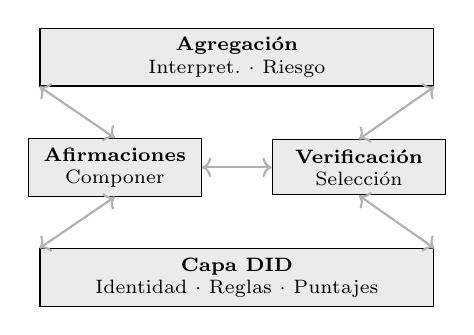
\begin{tikzpicture}[
    layer/.style={draw, minimum height=0.7cm, align=center, font=\scriptsize, fill=black!8},
    arr/.style={<->, thick, gray!60}
]
\node[layer, minimum width=5cm] (agg) at (0,2.8) {\textbf{Agregación}\\Interpret.\ $\cdot$ Riesgo};
\node[layer, minimum width=2.2cm] (claim) at (-1.55,1.4) {\textbf{Afirmaciones}\\Componer};
\node[layer, minimum width=2.2cm] (verif) at (1.55,1.4) {\textbf{Verificación}\\Selección};
\node[layer, minimum width=5cm] (did) at (0,0) {\textbf{Capa DID}\\Identidad $\cdot$ Reglas $\cdot$ Puntajes};

\draw[arr] (agg.south west) -- (claim.north);
\draw[arr] (agg.south east) -- (verif.north);
\draw[arr] (claim.east) -- (verif.west);
\draw[arr] (claim.south) -- (did.north west);
\draw[arr] (verif.south) -- (did.north east);
\end{tikzpicture}
\caption{Arquitectura de cuatro capas de la RSN.}
\label{fig:architecture}
\end{figure}

\subsection{Roles de los participantes}

Una transacción de verificación involucra hasta seis roles DID distintos (Fig.~\ref{fig:roles}): \textbf{Emisor} ($DID_I$, crea y presenta la afirmación), \textbf{Sujeto} ($DID_S$, el DID sobre el que trata la afirmación---puede coincidir con el Emisor), \textbf{Autoridad} ($DID_A$, respalda la afirmación a cambio de una tarifa; también puede ofrecer servicios de testigo---\emph{opcional}), \textbf{Testigo} ($DID_{W_{1..n}}$, monitor de incógnito de la honestidad del verificador mediante códigos de desafío---\emph{opcional}), \textbf{Verificador} ($DID_V$, seleccionado algorítmicamente para publicar la afirmación) y la \textbf{RSN} (la red donde se publican las afirmaciones verificadas). Cualquier rol puede delegarse en otro DID (Sección~7.4). Una Autoridad suele agrupar el respaldo con los servicios de testigo, pero ambas funciones son lógicamente independientes.

\begin{figure}[ht]
\centering
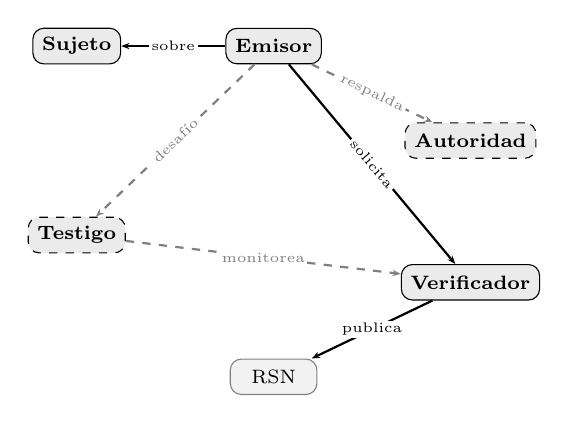
\begin{tikzpicture}[
    role/.style={draw, rounded corners, minimum width=1.1cm, minimum height=0.45cm, align=center, font=\scriptsize, fill=black!8},
    opt/.style={draw, rounded corners, minimum width=1.1cm, minimum height=0.45cm, align=center, font=\scriptsize, fill=black!8, dashed},
    arr/.style={-{Stealth[length=3pt]}, thick},
    oarr/.style={-{Stealth[length=3pt]}, thick, dashed, gray},
    lbl/.style={font=\tiny, fill=white, inner sep=1pt}
]
\node[role] (I) at (0,2.4) {\textbf{Emisor}};
\node[role] (S) at (-2.5,2.4) {\textbf{Sujeto}};
\node[opt] (A) at (2.5,1.2) {\textbf{Autoridad}};
\node[opt] (W) at (-2.5,0) {\textbf{Testigo}};
\node[role] (V) at (2.5,-0.6) {\textbf{Verificador}};
\node[role, fill=black!5, draw=gray] (N) at (0,-1.8) {RSN};

\draw[arr] (I) -- node[lbl] {sobre} (S);
\draw[oarr] (I) -- node[lbl,sloped] {respalda} (A);
\draw[oarr] (I) -- node[lbl,sloped] {desafío} (W);
\draw[arr] (I) -- node[lbl,sloped] {solicita} (V);
\draw[oarr] (W) -- node[lbl] {monitorea} (V);
\draw[arr] (V) -- node[lbl] {publica} (N);
\end{tikzpicture}
\caption{Roles DID en una transacción de verificación. Discontinuo = opcional (Autoridad, Testigo).}
\label{fig:roles}
\end{figure}

\subsection{Incorruptibilidad: cuatro fuerzas}

La incorruptibilidad de la RSN no surge de un único mecanismo, sino de cuatro fuerzas concurrentes. Ninguna es suficiente por sí sola; solo su combinación hace que un intento de corrupción resulte económicamente irracional.

\textbf{Objetivo impredecible.} El verificador de cada afirmación se selecciona de forma no determinista mediante hashing consistente (Sección~5.3). Un atacante no puede fijar de antemano a un verificador específico para sobornarlo, porque la identidad del verificador es función del contenido de la afirmación y de las iteraciones previas, no de la elección del emisor.

\textbf{Apalancamiento reputacional---sube lento, cae rápido.} La reputación solo puede ganarse de forma incremental, mediante un comportamiento coherente y sostenido. Sin embargo, puede perderse de forma catastrófica con un único respaldo fraudulento (Sección~6.2). Esta asimetría implica que años de reputación acumulada pueden destruirse con un solo respaldo deshonesto; la estrategia óptima sigue siendo rechazar las afirmaciones sospechosas.

\textbf{Promesa pública.} Cada Titular de un DID declara públicamente su política---un conjunto de reglas legibles por máquina que se compromete a cumplir. La divergencia entre la declaración y el comportamiento real es detectable y se penaliza como una falta reputacional más grave que la infracción subyacente (Sección~7.3). Por lo tanto, la hipocresía resulta más costosa que la deshonestidad directa.

\textbf{Asimetría de costo de ataque a la malla.} El costo de censurar o desestabilizar la red crece de forma no lineal con el tamaño y la densidad de la red, mientras que el costo de tolerarla permanece constante. Para que la censura rinda, un actor centralizado tendría que aplicarla en toda la red---lo que exige medidas desproporcionadas frente a cualquier beneficio concebible (Sección~10).

% ============================================================
% 4. DECENTRALIZED IDENTITY MODEL
% ============================================================
\section{Modelo de identidad descentralizada}

\subsection{DID con propiedades especiales}

La RSN amplía la especificación W3C DID Core~\cite{did2022} con: \textbf{Reglas Declaradas} (compromisos conductuales legibles por máquina), \textbf{Metadatos de Reputación} (puntaje conductual agregado) y \textbf{Enrutamiento de Red} (pasarela onion mutable, separada de la posición estable en el anillo).

\subsection{Ciclo de vida de una afirmación}

Una afirmación atraviesa seis etapas (Fig.~\ref{fig:lifecycle}): composición, respaldo opcional de autoridad, selección de verificador mediante hashing consistente, decisión de verificación (aceptar o rechazar con iteración), publicación y actualización de reputación para todas las partes.

\begin{figure}[ht]
\centering
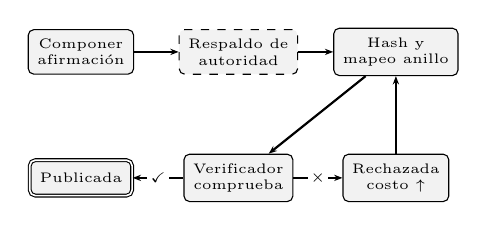
\begin{tikzpicture}[
    stp/.style={draw, rounded corners=2pt, minimum width=1.3cm, minimum height=0.45cm, align=center, font=\tiny, fill=black!5},
    arr/.style={-{Stealth[length=3pt]}, thick},
    lbl/.style={font=\tiny, fill=white, inner sep=1pt}
]
\node[stp] (comp) at (0,0) {Componer\\afirmación};
\node[stp, dashed] (auth) at (2.0,0) {Respaldo de\\autoridad};
\node[stp] (hash) at (4.0,0) {Hash y\\mapeo anillo};
\node[stp] (ver) at (2.0,-1.6) {Verificador\\comprueba};
\node[stp, double] (pub) at (0,-1.6) {Publicada};
\node[stp] (rej) at (4.0,-1.6) {Rechazada\\costo $\uparrow$};

\draw[arr] (comp) -- (auth);
\draw[arr] (auth) -- (hash);
\draw[arr] (hash) -- (ver);
\draw[arr] (ver) -- node[lbl] {\checkmark} (pub);
\draw[arr] (ver) -- node[lbl] {$\times$} (rej);
\draw[arr] (rej) -- ++(0,0.8) -| (hash);
\end{tikzpicture}
\caption{Ciclo de vida de una afirmación con bucle de iteración.}
\label{fig:lifecycle}
\end{figure}

\subsection{Relación con W3C DID Core}

El modelo de identidad de la RSN es un superconjunto propio de la especificación W3C DID Core~\cite{did2022}. Todos los DID de la RSN son DID válidos según W3C. Las extensiones específicas de la RSN se codifican como propiedades del documento DID definidas en una especificación de método DID dedicada, compatible con infraestructura existente como ION~\cite{buchner2021} y Ceramic~\cite{ceramic2023}.

% ============================================================
% 5. VERIFICATION AND PROPAGATION
% ============================================================
\section{Verificación y propagación de la información}

\subsection{Costo de ingreso de información}

El principio económico central de la RSN es la asimetría entre leer y escribir. Leer datos de reputación se acerca a un costo marginal nulo para los participantes que forman parte de la red DID y disponen de un acceso acorde con su reputación---los recién llegados deben ganar gradualmente un acceso más amplio (véase antiparasitismo). Escribir---entendido como la materialización duradera de la reputación en la red, no como un acto técnico puntual---requiere una inversión acumulada verificable en tres dimensiones: \textbf{tiempo} (años de vida dedicados a un comportamiento coherente, compromisos cumplidos y relaciones cultivadas), \textbf{energía} (esfuerzo invertido en actuar con honestidad, cuidar las asociaciones y mantener la confiabilidad a largo plazo) y \textbf{dinero} (inversión en el propio nombre---desarrollo profesional, calidad del propio trabajo, resarcimiento por los daños causados). La reputación no puede comprarse de forma instantánea---es el resultado de una acumulación de toda una vida que el sistema simplemente hace visible y transferible entre contextos. Los costos técnicos puntuales del protocolo (firmas criptográficas, tarifas de verificadores) son insignificantes frente a esta inversión subyacente.

\subsection{Grafo social y profundidad de contactos}

La RSN es, en esencia, una red social: cada DID agrega contactos (otros DID) que permiten la conexión. Esos contactos tienen sus propios contactos, y así sucesivamente. La búsqueda algorítmica de verificadores opera dentro de una profundidad configurable $h$ de contactos vinculados (por ejemplo, $h=3$: los contactos directos, sus contactos y los contactos de esos contactos). Esta arquitectura no requiere una única blockchain global---favorece de forma natural la aparición de comunidades/clústeres con solapamientos hacia otras comunidades. Todo participante DID debe tener una \textbf{política} publicada---un conjunto de reglas legibles por máquina que rige cómo se evalúan las solicitudes entrantes. Las violaciones de política se registran en la red como artefactos negativos.

\subsection{Selección algorítmica de verificadores}

El protocolo de verificación emplea hashing consistente~\cite{karger1997} (Fig.~\ref{fig:verifier}). La verificación es un servicio pagado: los verificadores operan a cambio de una tarifa, lo que crea un mercado donde la competencia impulsa el precio, la rapidez y la fiabilidad.

\textbf{Paso 1.} El documento de la afirmación se concatena con el resultado del hash de la iteración anterior (o $\varnothing$ en la primera iteración) y se aplica el hash:
\begin{equation}
\text{pos} = f_h(\text{claim} \| \text{prev\_hash})
\label{eq:hash}
\end{equation}

El algoritmo debe incluir la \emph{ruta completa} de todas las solicitudes y respuestas previas---no solo un hash de la iteración anterior. La respuesta completa de cada verificador (aceptación, rechazo, precio cotizado, motivo) se anexa al documento en crecimiento, verificable mediante firmas criptográficas en cada paso.

\textbf{Paso 2.} El hash se mapea a $N$ posiciones en el anillo de hashing consistente, distribuidas de forma uniforme (por ejemplo, para $N=4$: $+0^{\circ}, +90^{\circ}, +180^{\circ}, +270^{\circ}$). Desde cada posición, una búsqueda en sentido horario selecciona el DID más cercano como candidato a verificador (Fig.~\ref{fig:multipoint}). $N$ es un parámetro variable que puede depender del porcentaje de DID actualmente activos, de la hora del día o de la capacidad de respuesta histórica de la red.

\textbf{Paso 3.} El Verificador acepta (publica, arriesgando su reputación) o rechaza (regresando al Paso~1 con el hash del rechazo). Cuando un nodo no responde a pesar de declararse en línea, la siguiente solicitud debe incluir todas las respuestas de los $N$ candidatos a verificador anteriores.

\textbf{Antiparasitismo.} Los DID objetivo pueden fijar tarifas o restricciones de acceso para las consultas provenientes de DID nuevos con poca reputación. Este mecanismo graduado (no binario) obliga a los recién llegados a construir reputación mediante actividad genuina antes de consumir libremente los datos ajenos.

\begin{figure}[ht]
\centering
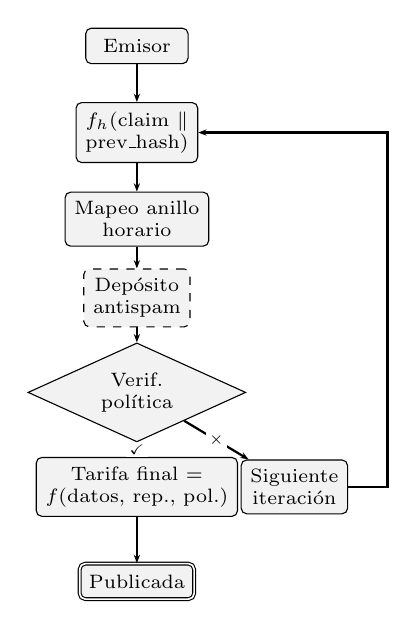
\begin{tikzpicture}[
    box/.style={draw, rounded corners=2pt, minimum width=1.3cm, minimum height=0.45cm, align=center, font=\scriptsize, fill=black!5},
    dec/.style={draw, diamond, aspect=2.2, minimum width=0.9cm, align=center, font=\scriptsize, fill=black!5},
    arr/.style={-{Stealth[length=3pt]}, thick},
    lbl/.style={font=\tiny, fill=white, inner sep=1pt}
]
\node[box] (iss) at (0,0) {Emisor};
\node[box] (hash) at (0,-1.1) {$f_h$(claim $\|$\\prev\_hash)};
\node[box] (ring) at (0,-2.2) {Mapeo anillo\\horario};
\node[box, dashed] (spam) at (0,-3.2) {Depósito\\antispam};
\node[dec] (check) at (0,-4.4) {Verif.\\política};
\node[box] (rej) at (2,-5.6) {Siguiente\\iteración};
\node[box] (fee) at (0,-5.6) {Tarifa final =\\$f$(datos, rep., pol.)};
\node[box, double] (pub) at (0,-6.8) {Publicada};

\draw[arr] (iss) -- (hash);
\draw[arr] (hash) -- (ring);
\draw[arr] (ring) -- (spam);
\draw[arr] (spam) -- (check);
\draw[arr] (check) -- node[lbl] {$\times$} (rej);
\draw[arr] (check) -- node[lbl] {\checkmark} (fee);
\draw[arr] (fee) -- (pub);
\draw[arr] (rej.east) -- ++(0.5,0) |- (hash.east);
\end{tikzpicture}
\caption{Protocolo de selección de verificadores. El depósito antispam es opcional y puede ser reembolsable. La tarifa final se paga solo en caso de aceptación.}
\label{fig:verifier}
\end{figure}

Cada rechazo anexa la respuesta completa del verificador (incluidos motivos y condiciones) al documento de la afirmación, ampliando su contenido. A partir del documento ampliado se calcula de forma no determinista un nuevo hash, que se mapea a una posición distinta del anillo y selecciona un verificador diferente. La documentación de la ruta completa es obligatoria---el emisor no puede predecir ni influir en el siguiente verificador. Si un verificador ignora una solicitud a pesar de tener una política declarada compatible, los testigos (si están presentes) lo registran, y el emisor puede adjuntar la evidencia de los testigos al momento de la publicación final.

\begin{figure}[ht]
\centering
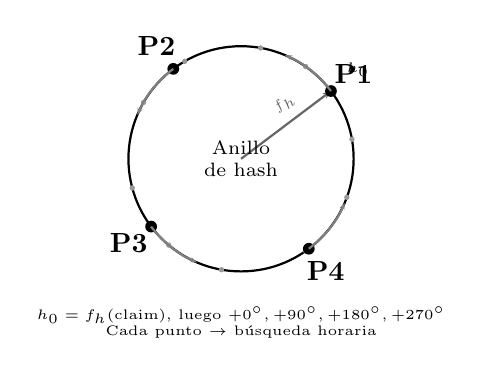
\begin{tikzpicture}[scale=0.65]
% Ring
\draw[thick] (0,0) circle (2.2cm);
% DID nodes on ring
\foreach \a in {10,55,80,120,150,195,230,260,305,340} {
  \fill[black!40] (\a:2.2) circle (1.5pt);
}
% Hash offset arrow pointing to initial position
\draw[-{Stealth[length=3pt]}, thick, black!60] (0,0) -- node[font=\tiny,above,sloped,pos=0.6] {$f_h$} (37:2.2);
\fill[black] (37:2.2) circle (2pt);
\node[font=\tiny,anchor=south west] at (37:2.35) {$h_0$};
% N=4 points offset from h0 by +0, +90, +180, +270
\foreach \offset/\l in {0/P1,90/P2,180/P3,270/P4} {
  \pgfmathsetmacro{\ang}{37+\offset}
  \node[fill=black, circle, inner sep=1.5pt] (p\offset) at (\ang:2.2) {};
  \node[font=\tiny,font=\bfseries] at (\ang:2.75) {\l};
  % clockwise search arc
  \draw[-{Stealth[length=2.5pt]}, thick, gray] (\ang:2.2) arc (\ang:\ang+30:2.2);
}
\node[font=\scriptsize, align=center] at (0,0) {Anillo\\de hash};
\node[font=\tiny, align=center] at (0,-3.2) {$h_0 = f_h(\text{claim})$, luego $+0^{\circ},+90^{\circ},+180^{\circ},+270^{\circ}$\\Cada punto $\rightarrow$ búsqueda horaria};
\end{tikzpicture}
\caption{Selección multipunto ($N{=}4$). El hash $h_0$ fija el desfase; 4 puntos distribuidos de forma uniforme desde $h_0$.}
\label{fig:multipoint}
\end{figure}

\subsection{Protocolo de testigos}

El rol de \textbf{Testigo} aporta responsabilidad de incógnito para la honestidad del verificador mediante un protocolo criptográfico de códigos de desafío:

\textbf{Paso W1.} El solicitante firma la solicitud de verificación y la envía a $N_w$ testigos---contactos de la red social del solicitante, o proveedores especializados de servicios de testigo que operan a cambio de una tarifa.

\textbf{Paso W2.} Cada testigo $w_i$ firma la solicitud firmada completa, conserva la firma original $\sigma_i$ y calcula un código de desafío $c_i = h(\sigma_i)$. El código de desafío se anexa a la solicitud.

\textbf{Paso W3.} La solicitud, que ahora porta $N_w$ códigos de desafío, se envía al verificador. El verificador observa los códigos pero \emph{no puede determinar} quiénes son los testigos ni si los códigos corresponden a firmas reales.

\textbf{Paso W4 (verificador honesto).} Si el verificador responde conforme a su política declarada, los códigos de desafío permanecen opacos. Los testigos nunca se revelan. No se publican datos adicionales.

\textbf{Paso W5 (violación de política).} Si el verificador viola su política (ignora la solicitud, responde de forma incoherente), el solicitante conserva las firmas originales de los testigos $\sigma_i$. Estas pueden publicarse como datos complementarios: cualquiera puede verificar $c_i = h(\sigma_i)$, probando que el testigo estuvo presente. El solicitante puede publicar de forma independiente---el verificador ya firmó los códigos de desafío en su respuesta.

\textbf{La propiedad del farol.} El solicitante puede sustituir por valores aleatorios algunos o todos los códigos de desafío. El verificador no puede distinguir los códigos genuinos (respaldados por autoridades de alta reputación) del ruido. Esta \emph{incertidumbre} es el mecanismo de ejecución: cada solicitud conlleva el riesgo de que una autoridad respetada esté observando de incógnito. El costo de mantener esta presión es casi nulo (generar números aleatorios), mientras que el costo potencial de la deshonestidad para el verificador es catastrófico. El comportamiento honesto se incentiva incluso en ausencia de testigos reales.

\textbf{La Autoridad como testigo.} Una Autoridad que respalda una afirmación puede agrupar servicios de testigo: ``Respaldo tu afirmación y actúo como testigo de incógnito durante la verificación.'' Este es un modelo de negocio natural---la Autoridad ya cuenta con el contexto. No obstante, los dos roles son lógicamente independientes.

\subsection{Principio del Radicalismo Costoso}

Tres canales de costo se acumulan simultáneamente (Fig.~\ref{fig:radicalism}):

\textbf{Canal 1: Costo de iteración.} Cada rechazo obliga a una nueva iteración que consume tiempo y recursos. Crecimiento lineal.

\textbf{Canal 2: Inflación del documento.} Cada iteración agrega la respuesta completa del verificador al documento de la afirmación. El crecimiento es lineal, pero con un desfase de base: la carga inicial (contenido de la afirmación, respaldo de autoridad, firmas criptográficas) ya tiene un tamaño no trivial $B_0$. Tamaño total tras $k$ iteraciones: $S(k) = B_0 + k \cdot \Delta$, donde $\Delta$ es el tamaño promedio de una respuesta.

\textbf{Canal 3: Prima de riesgo del verificador.} El riesgo es subjetivo. El verificador evalúa si las políticas declaradas del DID solicitante entran en conflicto con sus propios intereses comerciales, sociales o políticos. La prima puede escalar de forma exponencial con la distancia percibida respecto del ``ideal'' del verificador: $P(d) = \alpha \cdot e^{\beta d}$, donde $d$ es la métrica de distancia subjetiva del verificador. Más allá de un límite personal infranqueable, el verificador puede rechazar por completo.

\begin{figure}[ht]
\centering
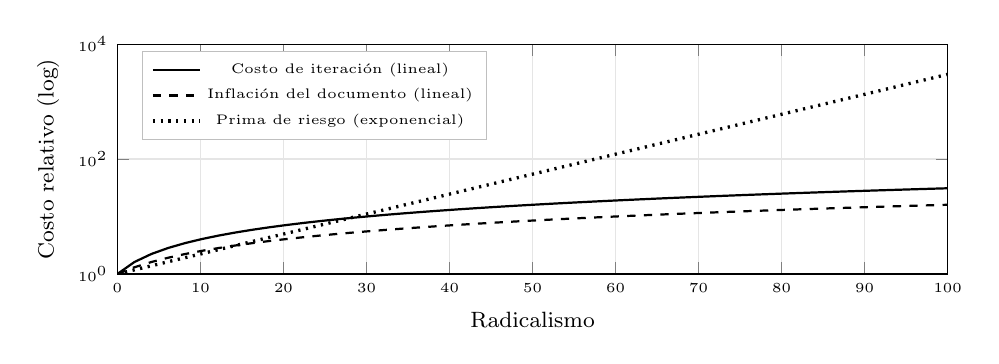
\begin{tikzpicture}
\begin{axis}[
    width=\columnwidth,
    height=4.5cm,
    xlabel={\footnotesize Radicalismo},
    ylabel={\footnotesize Costo relativo (log)},
    ymode=log,
    xmin=0, xmax=100,
    ymin=1, ymax=10000,
    grid=major,
    grid style={gray!20},
    legend style={at={(0.03,0.97)},anchor=north west,font=\tiny,draw=gray!50},
    tick label style={font=\tiny},
    label style={font=\footnotesize},
]
\addplot[black, thick, domain=0:100, samples=50] {1 + 0.3*x};
\addlegendentry{Costo de iteración (lineal)}
\addplot[black, thick, dashed, domain=0:100, samples=50] {1 + 0.15*x};
\addlegendentry{Inflación del documento (lineal)}
\addplot[black, thick, dotted, line width=1.2pt, domain=0:100, samples=100] {exp(0.08*x)};
\addlegendentry{Prima de riesgo (exponencial)}
\end{axis}
\end{tikzpicture}
\caption{Escalada de costos a través de tres canales. La prima de riesgo domina con radicalismo alto.}
\label{fig:radicalism}
\end{figure}

De manera crucial, esto no es censura. Ninguna afirmación se prohíbe. El sistema pone precio al riesgo (Tabla~\ref{tab:costs}).

\begin{table}[ht]
\centering
\caption{Comparación de costos según el tipo de afirmación.}
\label{tab:costs}
\footnotesize
\begin{tabular}{@{}lcccc@{}}
\toprule
\textbf{Tipo} & \textbf{Iter.} & \textbf{Doc} & \textbf{Tarifa} & \textbf{Total} \\
\midrule
Creíble & $k_{\min}$ & $B_0$ & $P_{\min}$ & Bajo \\
Controvertida & $k_{\text{med}}$ & $B_0{+}k\Delta$ & $\alpha e^{\beta d}$ & Moderado \\
Radical & $k_{\max}$ & $\gg B_0$ & $\gg P_{\min}$ & Muy alto \\
Fraudulenta & $\to\infty$ & --- & --- & Impublicable \\
\bottomrule
\end{tabular}
\end{table}

% ============================================================
% 6. REPUTATION AND RISK
% ============================================================
\section{Reputación y evaluación de riesgo}

\subsection{Modelo de acumulación de reputación}

La reputación exhibe tres propiedades: \textbf{acumulación lenta} (crecimiento incremental mediante un comportamiento coherente), \textbf{destrucción rápida} (un solo fraude puede reducir el puntaje de forma catastrófica) y \textbf{evaluación individual} (cada parte consumidora puede aplicar su propia función de agregación).

\subsection{Autoridades Reputables}

Una Autoridad Reputable revisa las afirmaciones y, si queda conforme, las cofirma---arriesgando su propia reputación (Fig.~\ref{fig:authority}). La asimetría es intencional: ganar reputación es lento (incremental $+\delta$ por cada respaldo honesto), mientras que perderla es catastrófico ($-\Delta \gg \delta$ por cada respaldo falso; a modo ilustrativo, por ejemplo, $+2\%$ frente a $-70\%$). La estrategia óptima es siempre rechazar las afirmaciones sospechosas. Los valores concretos de $\delta$ y $\Delta$ son parámetros del sistema.

\begin{figure}[ht]
\centering
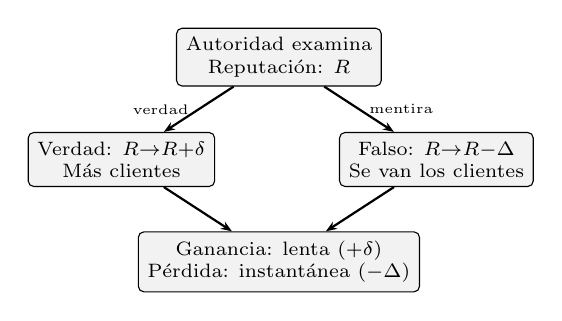
\begin{tikzpicture}[
    box/.style={draw, rounded corners=2pt, minimum width=2cm, minimum height=0.6cm, align=center, font=\scriptsize, fill=black!5},
    arr/.style={-{Stealth[length=4pt]}, thick}
]
\node[box] (exam) at (0,0) {Autoridad examina\\Reputación: $R$};
\node[box] (true) at (-2,-1.3) {Verdad: $R{\to}R{+}\delta$\\Más clientes};
\node[box] (false) at (2,-1.3) {Falso: $R{\to}R{-}\Delta$\\Se van los clientes};
\node[box] (insight) at (0,-2.6) {Ganancia: lenta ($+\delta$)\\Pérdida: instantánea ($-\Delta$)};

\draw[arr] (exam) -- node[left,font=\tiny] {verdad} (true);
\draw[arr] (exam) -- node[right,font=\tiny] {mentira} (false);
\draw[arr] (true) -- (insight);
\draw[arr] (false) -- (insight);
\end{tikzpicture}
\caption{Autoridad Reputable---incentivos asimétricos.}
\label{fig:authority}
\end{figure}

\subsection{Reputación multidimensional}

La reputación no es un escalar, sino un vector a lo largo de múltiples dimensiones: fiabilidad financiera, integridad personal, competencia profesional, participación cívica y otras (Fig.~\ref{fig:reputation-radar}). Distintos proveedores de evaluación proyectan este vector de manera diferente según el contexto---un prestamista prioriza la fiabilidad financiera, un empleador la competencia profesional, un vecino el comportamiento cívico. No existe un único puntaje de reputación ``correcto''; solo perspectivas.

\begin{figure}[ht]
\centering
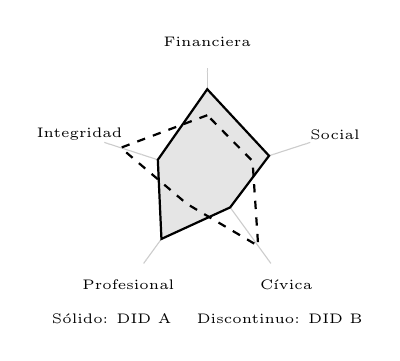
\begin{tikzpicture}[scale=0.55]
\foreach \a/\l in {90/Financiera,162/Integridad,234/Profesional,306/Cívica,18/Social} {
  \draw[gray!40] (0,0) -- (\a:2.5);
  \node[font=\tiny, align=center] at (\a:3.1) {\l};
  \foreach \r in {0.8,1.6,2.4} {
    \fill[black!15] (\a:\r) circle (0.5pt);
  }
}
\draw[thick, fill=black!10] (90:2.0) -- (162:1.2) -- (234:1.8) -- (306:0.9) -- (18:1.5) -- cycle;
\draw[thick, dashed] (90:1.4) -- (162:2.1) -- (234:0.8) -- (306:2.0) -- (18:1.1) -- cycle;
\node[font=\tiny] at (0,-3.3) {Sólido: DID A \quad Discontinuo: DID B};
\end{tikzpicture}
\caption{Vectores de reputación multidimensional. Distintos DID exhiben perfiles diferentes entre las dimensiones.}
\label{fig:reputation-radar}
\end{figure}

\subsection{Evaluación de riesgo democratizada}

La RSN democratiza la evaluación sistemática de riesgo---una capacidad hoy concentrada en las instituciones financieras, pero aplicable mucho más allá de la banca. Conglomerados industriales que evalúan la fiabilidad de sus proveedores, compañías de seguros que ponen precio al riesgo conductual, la debida diligencia en fusiones y adquisiciones, la estimación de la vida útil de equipos en la manufactura---dondequiera que el riesgo de contraparte requiera evaluación, la RSN ofrece una alternativa descentralizada e impulsada por el mercado. Un mercado de servicios de interpretación traduce los datos brutos de reputación multidimensional en resúmenes accionables, haciendo que la evaluación de contrapartes sea accesible para cualquier participante a un costo marginal.

% ============================================================
% 7. CONSENSUS AND DISPUTE RESOLUTION
% ============================================================
\section{Consenso y resolución de disputas}

\subsection{Modelo de justicia descentralizada}

La RSN replantea la justicia como un problema de negociación bilateral. La amenaza de un daño reputacional permanente y verificable es un disuasivo más eficaz que un proceso judicial que la parte perjudicada no puede costear.

\subsection{Consenso emergente}

Cada participante mantiene un umbral personal de satisfacción. El consenso agregado de la red emerge como el promedio estadístico de miles de negociaciones bilaterales (Fig.~\ref{fig:consensus}). Una respuesta muy por encima del consenso (bárbara) es cara de publicar. Una respuesta cercana al consenso (proporcional) es barata. El consenso no es una regla---es una señal de precio.

\begin{figure}[ht]
\centering
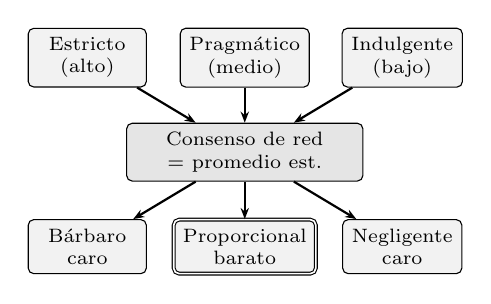
\begin{tikzpicture}[
    person/.style={draw, rounded corners=2pt, minimum width=1.5cm, minimum height=0.5cm, align=center, font=\scriptsize, fill=black!5},
    arr/.style={-{Stealth[length=4pt]}, thick}
]
\node[person] (a) at (-2,0) {Estricto\\(alto)};
\node[person] (b) at (0,0) {Pragmático\\(medio)};
\node[person] (c) at (2,0) {Indulgente\\(bajo)};
\node[person, fill=black!10, minimum width=3cm] (cons) at (0,-1.2) {Consenso de red\\= promedio est.};
\node[person] (exp) at (-2,-2.4) {Bárbaro\\caro};
\node[person, double] (prop) at (0,-2.4) {Proporcional\\barato};
\node[person] (neg) at (2,-2.4) {Negligente\\caro};

\draw[arr] (a) -- (cons);
\draw[arr] (b) -- (cons);
\draw[arr] (c) -- (cons);
\draw[arr] (cons) -- (exp);
\draw[arr] (cons) -- (prop);
\draw[arr] (cons) -- (neg);
\end{tikzpicture}
\caption{Consenso emergente a partir de umbrales individuales de satisfacción.}
\label{fig:consensus}
\end{figure}

\subsection{Calibración del castigo}

Cada Titular de un DID declara públicamente sus respuestas a categorías específicas de mala conducta. Las declaraciones desproporcionadamente duras o indulgentes atraen señales de reputación negativa. Las declaraciones proporcionales se aceptan sin fricción---un sistema de castigo autocalibrado.

Las declaraciones de consenso están a su vez sujetas a la detección de hipocresía: comprometerse declarativamente con una posición de consenso mientras se actúa de forma incoherente constituye una falta reputacional más grave que la desviación subyacente, ya que demuestra un engaño intencional.

\subsection{Delegación}

Todas las actividades dentro de un DID---con una excepción---pueden delegarse en otro DID. \textbf{El rol de Sujeto---el DID cuyo comportamiento describe la afirmación---no puede delegarse; está ligado de forma intransferible al titular de identidad al que se refiere la afirmación.} Los demás roles activos---Emisor, Autoridad, Testigo, Verificador---pueden transferirse a un DID delegado designado, ya sea para verificación, presentación de afirmaciones, participación en el consenso o resolución de disputas. La delegación es revocable en cualquier momento. Esto habilita la especialización (por ejemplo, servicios profesionales de verificación) mientras el Titular conserva el control y la responsabilidad últimos. La delegación se aplica en todo el sistema y es esencial para la escalabilidad.

\subsection{De la moral individual al contrato social emergente}

La política declarada de cada DID representa una formalización de la moral individual: qué considera aceptable el Titular, cómo responde a comportamientos específicos, qué exige de sus contrapartes. Estas políticas no las impone un diseñador del sistema---las elige cada participante y se expresan en forma legible por máquina.

Esta formalización habilita una emergencia en tres etapas. Primero, la moral individual se codifica como \textbf{política}---un conjunto de reglas declaradas, umbrales y funciones de respuesta que el DID se compromete a cumplir. Segundo, el agregado de todas las políticas a lo largo de la red produce una \textbf{ética emergente}---normas estadísticamente observables que ningún participante diseñó, pero que surgen de la interacción de miles de posiciones morales individuales~\cite{durkheim1893}. Tercero, esta ética emergente, expresada como normas de comportamiento compartidas que se hacen valer mediante señales de precio bilaterales, constituye un \textbf{contrato social medible}---no una construcción teórica que nadie firmó~\cite{rawls1971}, sino un conjunto de reglas observable empíricamente y respaldado por el comportamiento real.

Este proceso refleja los hallazgos de la teoría de los fundamentos morales~\cite{haidt2012}: la moral humana es intuitiva, pluralista y culturalmente variable. La RSN no requiere el consenso moral como insumo; produce el consenso conductual como resultado. El contrato social resultante no es estático---evoluciona a medida que los participantes se incorporan, se retiran y ajustan sus políticas en respuesta a la retroalimentación de la red. A diferencia de la teoría clásica del contrato social, este contrato es revocable, observable y ejecutable sin un soberano.

% ============================================================
% 8. ECONOMIC MODEL
% ============================================================
\section{Modelo económico}

Las secciones anteriores describieron una herramienta---los mecanismos de verificación, la estructura de costos y el consenso emergente de la RSN. Esta sección describe una metodología para aplicar esa herramienta a la transición fiscal y de gobernanza. La herramienta es de propósito general; la metodología que sigue es una aplicación posible.

\subsection{Estructura de incentivos}

La reputación como capital crea incentivos directos para el comportamiento honesto. En operación normal, los participantes construyen reputación de forma natural mediante transacciones cotidianas y compromisos cumplidos. El principal gasto recae en las afirmaciones \emph{negativas}---dejar constancia del daño causado por otros. Esta asimetría incentiva un comportamiento útil y fiable: ser honesto no cuesta nada adicional, mientras que ser dañino crea un rastro documentado que otros pagarán por preservar. La hipocresía---declarar reglas sin cumplirlas---es el modo de fallo más costoso, ya que demuestra un engaño intencional.

\subsection{Sistema fiscal paralelo}

Tres componentes habilitan la presión competitiva: (1)~\textbf{Impuesto Simple}---una única tasa proporcional sin excepciones, inicialmente apenas por debajo de la tasa efectiva vigente; (2)~\textbf{Registro Electrónico del Gasto (REG)}---que invierte el modelo checo EET para que los ciudadanos vigilen los gastos del Estado; (3)~\textbf{Asignación Tributaria Dirigida por el Ciudadano}---que comienza en un pequeño porcentaje el primer año y alcanza, tras una década, desde cifras de dos dígitos bajos hasta una migración total a un sistema dirigido por el ciudadano, según el ritmo de adopción. El tempo real depende de la velocidad con que surjan alternativas de libre mercado a los servicios estatales y de la disposición del Estado a cooperar con la transición; la función del tiempo no tiene por qué ser lineal, y no hay razón para fijar un límite superior a dónde puede llegar en última instancia la adopción.

% ============================================================
% 9. MIGRATION PATH
% ============================================================
\section{Vía de migración}

La migración avanza a través de tres fases (Fig.~\ref{fig:migration}): \textbf{Fase~1: Superposición} (la RSN como capa informativa, el Estado es el único proveedor), \textbf{Fase~2: Competencia} (la RSN ofrece alternativas funcionales, uso de doble sistema) y \textbf{Fase~3: Transición} (la RSN supera a los equivalentes estatales, migración voluntaria). La transición es reversible en cada etapa.

\begin{figure}[ht]
\centering
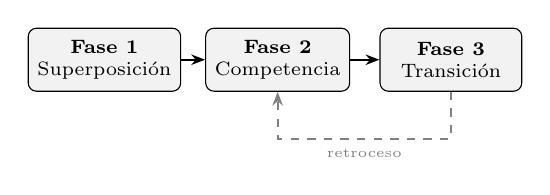
\begin{tikzpicture}[
    phase/.style={draw, rounded corners=3pt, minimum width=1.8cm, minimum height=0.8cm, align=center, font=\scriptsize, fill=black!5},
    arr/.style={-{Stealth[length=5pt]}, thick}
]
\node[phase] (p1) at (0,0) {\textbf{Fase 1}\\Superposición};
\node[phase] (p2) at (2.2,0) {\textbf{Fase 2}\\Competencia};
\node[phase] (p3) at (4.4,0) {\textbf{Fase 3}\\Transición};

\draw[arr] (p1) -- (p2);
\draw[arr] (p2) -- (p3);
\draw[arr, dashed, gray] (p3.south) -- ++(0,-0.6) -| node[below,font=\tiny,pos=0.25] {retroceso} (p2.south);
\end{tikzpicture}
\caption{Migración en tres fases---reversible en cada etapa.}
\label{fig:migration}
\end{figure}

El principal mecanismo de presión es fiscal: cuando los contribuyentes condicionales alcanzan una ``minoría económicamente significativa $X$''---un grupo lo bastante grande como para que la represión contra él cause un daño económico no trivial y la desobediencia civil se vuelva una amenaza creíble---, el Estado entra en negociación. A modo ilustrativo, usamos $X \approx 15\%$ del PIB, pero el umbral real depende de la economía específica.

% ============================================================
% 10. SECURITY ANALYSIS
% ============================================================
\section{Análisis de seguridad}

Consideramos cinco categorías de adversarios: malos actores individuales, grupos organizados, adversarios corporativos, adversarios a nivel estatal y adversarios a nivel de protocolo.

\textbf{Resistencia a Sybil}~\cite{douceur2002}. Construir reputación requiere una interacción sostenida y verificable. El costo de un ataque Sybil exitoso escala linealmente con las identidades falsas y cuadráticamente con el nivel de reputación objetivo. Operar múltiples DID en paralelo es posible pero, por diseño, costoso---cada identidad debe acumular reputación de forma independiente mediante actividad genuina. En las sociedades libres, este costo disuade el abuso ocasional; en las dictaduras, los DID paralelos se convierten en una herramienta de supervivencia que habilita la resistencia compartimentada, la coordinación clandestina y una navegación más segura del mercado negro.

\textbf{Defensa contra la colusión.} Los patrones de respaldo mutuo entre grupos cerrados son detectables mediante el análisis del grafo social. Las funciones de agregación de reputación descuentan las afirmaciones provenientes de fuentes densamente agrupadas.

\textbf{Adversario a nivel estatal.} El enrutamiento onion, la ausencia de infraestructura centralizada y la distribución del rol de Verificador entre la base de participantes garantizan que la supresión requiera medidas desproporcionadas frente a cualquier beneficio.

\textbf{Privacidad frente a rendición de cuentas.} La seudonimia---un punto intermedio entre el anonimato y la divulgación de identidad---permite que los DID acumulen una reputación significativa sin revelar la identidad real del Titular.

% ============================================================
% 11. PRIVACY
% ============================================================
\section{Consideraciones de privacidad}

El modelo de privacidad de la RSN se construye sobre la seudonimia. El Titular controla la divulgación de identidad: mínima (seudónimo puro), selectiva (credenciales específicas vinculadas) o total (identidad legal asociada). Las afirmaciones publicadas son permanentes---el sistema admite la corrección contextual pero no el borrado. Un Titular puede abandonar un DID comprometido y empezar de nuevo, renunciando a la reputación acumulada.

% ============================================================
% 12. RELATED WORK
% ============================================================
\section{Trabajos relacionados}

La especificación W3C DID Core~\cite{did2022} y la red Ceramic~\cite{ceramic2023} aportan la base de identidad. EigenTrust~\cite{kamvar2003} demostró la agregación distribuida de reputación sin autoridad central. Los SBT~\cite{weyl2022} introdujeron tokens sociales intransferibles. La RSN se distingue por su énfasis en el costo económico como filtro de calidad y por su mecanismo para poner precio al radicalismo.

Las DAO~\cite{buterin2014} y la votación cuadrática~\cite{buterin2019} demostraron la viabilidad de la gobernanza descentralizada. La RSN deriva el consenso de negociaciones de precio bilaterales en lugar de la votación.

La propuesta se apoya en la teoría anarcocapitalista~\cite{rothbard1973,hoppe2001} para la provisión privada de servicios, pero se aparta de ella en dos aspectos críticos: diseña para el rencor y los impulsos retributivos en lugar de suponer racionalidad, y propone una transición gradual en lugar de una revolución. El concepto de contratos sociales emergentes tiene antecedentes en la teoría del orden espontáneo de Hayek~\cite{hayek1973}.

\textbf{Anarcoagorismo.} La RSN comparte un terreno común importante con la contraeconomía agorista~\cite{konkin2006}---en particular el énfasis en construir instituciones paralelas y el intercambio voluntario. Sin embargo, el agorismo tiende a suponer el interés propio racional como mecanismo de coordinación suficiente y a menudo carece de una vía de migración concreta desde las estructuras estatales existentes. La RSN incorpora explícitamente tendencias conductuales no racionales y aporta un mecanismo de presión fiscal para una transición gradual.

\textbf{Meritocracia.} La RSN puede representar una primera descripción funcional de cómo la meritocracia~\cite{young1958} puede emerger como una propiedad sistémica en lugar de un eslogan. Los sistemas meritocráticos tradicionales fracasan porque requieren una autoridad central que defina y haga valer el ``mérito''. En la RSN, el mérito emerge de evaluaciones bilaterales: quienes aportan valor acumulan reputación; ningún comité decide quién tiene mérito.

\textbf{La propiedad como privilegio.} La RSN se aparta de forma fundamental de los tratamientos anarcocapitalistas y de la escuela austríaca sobre los derechos de propiedad como naturales y absolutos. En el marco de la RSN, la propiedad es un \emph{privilegio}---un reconocimiento social que, en casos extremos, puede ser retirado por la comunidad cuando un participante viola de forma fundamental las normas compartidas (traición, negativa a defender a la comunidad en una crisis existencial, explotación sistemática). Esto no es expropiación estatal, sino un retiro del reconocimiento social por parte de la red de relaciones bilaterales.

% ============================================================
% 13. LIMITATIONS
% ============================================================
\section{Discusión y limitaciones}

\textbf{Arranque en frío.} El valor de la RSN depende de los efectos de red; quienes la adoptan temprano enfrentan un valor limitado hasta que la participación alcanza un umbral. No obstante, incluso desde etapas tempranas, la red DID sirve como una fuente de información complementaria útil. Se espera que la evaluación temprana de reputación y de autoridades se desarrolle de forma gradual, con creciente sofisticación.

\textbf{Antiparasitismo y control de acceso.} Los DID objetivo pueden imponer tarifas graduadas y restricciones de acceso a las consultas provenientes de DID de baja reputación. Esto no es binario, sino una escala continua: cuanta menos reputación tenga un DID consultante, menos información recibe, más espera y más paga. Este mecanismo incentiva la participación genuina por encima del consumo pasivo.

\textbf{Desigualdad de acceso.} El costo de publicar afirmaciones puede filtrar quejas legítimas de participantes económicamente desfavorecidos. Mitigación: todo participante actúa simultáneamente como verificador potencial (o delega ese rol) y gana tarifas de verificación. En un horizonte temporal suficiente, un participante no radical debería aproximarse a la neutralidad financiera---sus ingresos por verificación compensarían aproximadamente los costos de publicación. Esta es una expectativa estadística, no una garantía.

\textbf{Desigualdad de reputación.} Quienes adoptan la red temprano acumulan ventajas que pueden crear barreras para los rezagados. Sin embargo, la evaluación de reputación la realizan proveedores externos que pueden optar por mitigar la ventaja del primero en mover mediante sus algoritmos de agregación. Ser el primero con una buena reputación es una ventaja económica comparativa legítima---y eso es intencional.

\textbf{Preguntas abiertas.} Las funciones de costo óptimas, los estándares de agregación, la gobernanza del protocolo y la interacción con datos de reputación sintética generados por IA siguen siendo áreas para trabajo futuro.

Este artículo no afirma que la RSN vaya a producir resultados óptimos en todas las circunstancias. Afirma que la RSN representa una alternativa \emph{factible}---técnicamente implementable, económicamente autosostenible y socialmente compatible con las tendencias conductuales humanas tal como son en realidad.

% ============================================================
% 14. CONCLUSION
% ============================================================
\section{Conclusión}

Este artículo ha presentado la Red Social de Reputación, un protocolo descentralizado que habilita el intercambio de reputación seudónimo y verificable. El Principio del Radicalismo Costoso garantiza que las afirmaciones fraudulentas queden fuera de precio sin censura. La vía de migración propuesta habilita una transición gradual y reversible desde las instituciones existentes. El diseño incorpora la naturaleza humana tal como es---incluidas la mezquindad, el rencor y el deseo de satisfacción retributiva---en lugar de exigir una transformación ideológica. El resultado no es una utopía, sino un sistema donde la justicia es accesible, la reputación se gana y el costo de la mala conducta lo asume la parte que lo causó.

% ============================================================
% REFERENCES
% ============================================================
\bibliography{references}

\end{document}
